\documentclass[
%a4paper,12pt
encoding=utf8
]{twoeskd}

% Packages required by doxygen
\usepackage{fixltx2e}
\usepackage{calc}
\usepackage{doxygen}
\usepackage[export]{adjustbox} % also loads graphicx
\usepackage{graphicx}
\usepackage[utf8]{inputenc}
\usepackage{makeidx}
\usepackage{multicol}
\usepackage{multirow}
\PassOptionsToPackage{warn}{textcomp}
\usepackage{textcomp}
\usepackage[nointegrals]{wasysym}




% NLS support packages
\usepackage[T2A]{fontenc}
\usepackage[russian]{babel}

% Font selection
\usepackage{courier}
\usepackage{amssymb}
\usepackage{sectsty}
\renewcommand{\familydefault}{\sfdefault}
\newcommand{\+}{\discretionary{\mbox{\scriptsize$\hookleftarrow$}}{}{}}

% Page & text layout
\usepackage{geometry}
\tolerance=750
\hfuzz=15pt
\hbadness=750
\setlength{\emergencystretch}{15pt}
\setlength{\parindent}{0cm}
\setlength{\parskip}{0.2cm}
\makeatletter
\makeatother

% Headers & footers
% \usepackage{fancyhdr}
% \renewcommand{\sectionmark}[1]{%
%   \markright{\thesection\ #1}%
% }

% Indices & bibliography
\usepackage{natbib}
\usepackage[titles]{tocloft}
\setcounter{tocdepth}{3}
\setcounter{secnumdepth}{5}
\makeindex

\newcommand\tab[1][1cm]{\hspace*{#1}}
\usepackage{hyperref}
\hypersetup{
	colorlinks,
	citecolor=black,
	filecolor=black,
	linkcolor=black,
	urlcolor=black
}
% Custom commands
\newcommand{\clearemptydoublepage}{%
  \newpage{\pagestyle{empty}\cleardoublepage}%
}
\renewcommand{\DoxyLabelFont}{%
  \fontseries{bc}\selectfont%
}
\newcommand\degr{$^\circ$}

% Custom packages
\usepackage{pdfpages}


\setlength{\parindent}{0cm}
\setlength{\parskip}{0.2cm}

\usepackage{listings}

% debug to see the frame borders
% from https://en.wikibooks.org/wiki/LaTeX/Page_Layout
% \usepackage{showframe}

% change style of titles in \section{}
\usepackage{titlesec}
\titleformat{\section}[hang]{\huge\bfseries\center}{\thetitle.}{1em}{}
\titleformat{\subsection}[hang]{\Large\raggedright}{\thetitle.}{1em}{\underline}
\titleformat{\subsubsection}[hang]{\large\raggedright}{\thetitle.}{1pt}{}

% Packages for text layout in normal mode
% \usepackage[parfill]{parskip} % автоматом делает пустые линии между параграфами, там где они есть в тексте
% \usepackage{indentfirst} % indent even in first paragraph
\usepackage{setspace}	 % controls space between lines
\setstretch{1} % space between lines
\setlength\parindent{0.9cm} % size of indent for every paragraph
\usepackage{csquotes}% превратить " " в красивые двойные кавычки
\MakeOuterQuote{"}


% this makes items spacing single-spaced in enumerations.
\newenvironment{my_enumerate}{
\begin{enumerate}
  \setlength{\itemsep}{1pt}
  \setlength{\parskip}{0pt}
  \setlength{\parsep}{0pt}}{\end{enumerate}
}


% Custom commands
% configure eskd
\titleTop{
\textbf{\Large ПРАВИТЕЛЬСТВО РОССИЙСКОЙ ФЕДЕРАЦИИ \\
НАЦИОНАЛЬНЫЙ ИССЛЕДОВАТЕЛЬСКИЙ УНИВЕРСИТЕТ \\
«ВЫСШАЯ ШКОЛА ЭКОНОМИКИ» } \\
\vspace*{0.2cm}
{\small Факультет компьютерных наук \\
Департамент программнoй инженерии \\
}
}
\titleDesignedBy{Студент группы БПИ 151 НИУ ВШЭ}{Куприянов К.И.}
\titleAgreedBy{%
\parbox[t]{7cm} {
Доцент департамента \\
программной инженерии \\
факультета компьютерных наук \\
канд. техн. наук \\
}}{Гринкруг Е. М.}
\titleApprovedBy{
\parbox[t]{10cm} {
Академический руководитель \\
образовательной программы \\
«Программная инженерия» \\
профессор департамента программной \\
инженерии канд. техн. наук \\
}}{Шилов В. В.}
\titleName{Игра — Эскейп Квест с Использованием Очков Виртуальной Реальности}
\workTypeId{RU.17701729.509000 81 01-1}

\titleSubname{Пояснительная записка}


%===== C O N T E N T S =====
\begin{document}

% Titlepage & ToC
\pagenumbering{arabic}

\section{Аннотация}

\tab[0.75cm] Техническое задание – это основной документ, оговаривающий набор требований и
порядок создания программного продукта, в соответствии с которым производится разработка
программы, ее тестирование и приемка.

Настоящее Техническое задание на разработку ``Клиент-Серверное Android-Приложение для Управления Скидками в Розничных Сетях'' содержит следующие разделы: ``Введение'', ``Основания для разработки'',
``Назначение разработки'', ``Требования к программе'', ``Требования к программным документам'',
``Технико-экономические показатели'', ``Стадии и этапы разработки'', ``Порядок контроля и
приемки'' и приложения.

В разделе ``Введение'' указано наименование и краткая характеристика области применения
``Клиент-Серверного Android-Приложения для Управления Скидками в Розничных Сетях''.

В разделе ``Основания для разработки'' указан документ на основании, которого ведется
разработка и наименование темы разработки.

В разделе ``Назначение разработки'' указано функциональное и эксплуатационное
назначение программного продукта.

Раздел ``Требования к программе'' содержит основные требования к функциональным
характеристикам, к надежности, к условиям эксплуатации, к составу и параметрам технических
средств, к информационной и программной совместимости, к маркировке и упаковке, к
транспортировке и хранению, а также специальные требования.

Раздел ``Требования к программным документам'' содержит предварительный состав
программной документации и специальные требования к ней.

Раздел ``Технико-экономические показатели'' содержит ориентировочную экономическую
эффективность, предполагаемую годовую потребность, экономические преимущества разработки
``Клиент-Серверного Android-Приложения для Управления Скидками в Розничных Сетях''.

Раздел ``Стадии и этапы разработки'' содержит стадии разработки, этапы и содержание
работ.

В разделе ``Порядок контроля и приемки'' указаны общие требования к приемке работы.

Настоящий документ разработан в соответствии с требованиями:\\
1) ГОСТ 19.101-77 Виды программ и программных документов \cite{gost_types_of_software};\\
2) ГОСТ 19.102-77 Стадии разработки \cite{gost_stages_of_devel};\\
3) ГОСТ 19.103-77 Обозначения программ и программных документов \cite{gost_marking_software};\\
4) ГОСТ 19.104-78 Основные надписи \cite{gost_main_signs};\\
5) ГОСТ 19.105-78 Требования к программным документам \cite{gost_demands_for_docs};\\
6) ГОСТ 19.201-78 Техническое задание. Требования к содержанию и оформлению \cite{gost_tz}.\\

Изменения к данному Техническому заданию оформляются согласно ГОСТ 19.603-78 \cite{gost_main_rules_change},
Перед прочтением данного документа рекомендуется ознакомиться с терминологией,
приведенной в Приложении 1 настоящего технического задания.


\newpage
\pagenumbering{arabic}
\tableofcontents
% \pagenumbering{arabic}

% --- add my custom headers ---
\newpage
\section{Введение}
\subsection{Наименование программы}
Наименование программы на русском:
``Клиент-Серверное Android-Приложение для Управления Скидками в Розничных
Сетях''. \\
Наименование на английском:
``The Client-Server Android Application for Managing the Products' Discounts in
Retail Networks''.


\subsection{Краткая характеристика}
Программа предназначена для пользователей смартфонов на базе платформы Android.
Цель работы - создать удобное приложения для составления списков покупок,
добавления в них любых товаров (даже тех, которых нет в магазине), отслеживания
акций, а так же просмотра всех акций в нескольких магазинах. Это позволит
пользователям экономить свои средства на ежедневных покупках и быть в курсе
актуальных акций магазинов.  Серверная часть приложения должна представлять из
себя web-crawler для сбора данных с сайтов розничных сетей. Crawler должен
иметь модульную структуру, для быстрого восстановления после изменения дизайна
сайтов. Должен быть реализован механизм взаимодействия с клиентами посредством
обменивания файлами в формате JSON.\\
Главной чертой данного приложения
является его лёгкая, быстрая масштабируемость и модульность программного кода.



\newpage
\section{Назначение разработки}
\subsection{Функциональное назначение}
Продукт является приложением ``на стыке онлайна и оффлайна'', позволяющим планировать
покупки в магазине с учетом актуальных скидок. 
К функциональным возможностям программы относятся:
просмотр списка актуальных акций,
составление и редактирование списка покупок, 
поиск ближайшего магазина на карте,
регистрация пользователей,
возможность отправки списка покупок между пользователями.

\subsection{Эскплутационное назначение}
Программа предназначена для запуска на персональных компьютерах (веб-версия) и 
мобильных устройствах (веб-версия). Программа является 
приложением, позволяющим пользователю искать и подбирать интересующие его товары 
по сниженной цене, и, таким образом, экономить средства. 


% EOF



\newpage
\section{Технические характеристики}
\subsection{Постановка задачи на разработку программы}
\tab[0.75cm]Программа должна соответствовать требованиям, представленным в
Техническом
Задании.

\bigskip
\subsubsection{Задачи работы (Андроид-клиент)}
\smallskip
\begin{my_enumerate}
\item Реализовать возможность просмотра списка доступных магазинов с акционными товарами
\item Реализовать представление текущих акций для конкретного магазина:
    \begin{my_enumerate}
    \item В виде общего списка
    \item По категориям
    \end{my_enumerate}
\item Реализовать постепенную загрузку товаров магазинов (по страницам) для экономии трафика и меньшей нагрузкой на мобильное устройство
\item Реализовать регистрацию через мобильное приложение
\item Реализовать вход в аккаунт через мобильное приложение
\item Реализовать возможность смены аккаунта
\item Реализовать возможность создания списков покупок c разными названиями
\item Реализовать возможность удаления списка покупок
\item Реализовать возможность добавления товара в список покупок
\item Реализовать возможность удаления товара из списка покупок
\item Реализовать возможность добавления в список покупок пользовательских товаров, котороых нет в магазине (см. терминологию)
\item Реализовать возможность просмотра подобранных программой товаров согласно запросу пользователя
\item Реализовать добавление подобранных товаров в список покупок
\item Реализовать предварительное отображение элементов каждого списка покупок до их открытия
\item Реализовать отображение всплывающих подсказок при долгом нажатии на элементы управления button (кнопка)
\item Реализовать перенаправление в настройки сети для последующего включения интернета при отсутствии интернет-соединения
\item Реализовать отображение индикатора процесса загрузки данных с сервера
\item Реализовать обучающий фрагмент в разделе help (см. терминологию), содержащий руководство пользователя по управлению программой
\end{my_enumerate}

\subsubsection{Задачи работы (серверная часть)}

\smallskip
\begin{my_enumerate}
    \item Реализовать crawling веб-страниц для сбора актуальной информации об акционных товарах
        \begin{my_enumerate}
            \item Реализовать spider для каждого магазина для сбора данных с их веб-страниц
            \item Реализовать модуль text\_processor для очистки собранных текстовых данных
            \item Реализовать ``модульные'' xpath селекторы, для оперативного восстановления при изменении дизайна сайта
        \end{my_enumerate}
    \item Модуль pipelines: реализовать добавление товаров в базу данных посредством отправки запросов REST API (REST API и база данных реализованы напарником)
    \item Модуль pipelines: реализовать запись акционных товаров со всех магахинах в JSON файл
    \item Реализовать email уведомления администраторам сервиса об ошибках и неполадках в работе сервера
    \item Реализовать ежедневное обновление акций для поддержания актуальности
\end{my_enumerate}


\subsection{Описание алгоритма и функционирования программы}

\subsubsection{Описание построения Андроид приложения}
В андроид приложении задумано 4 активности (см. терминологию) и 2 фрагмента (см. терменологию)\\
\begin{my_enumerate}
    \item \textbf{LoginActivity} Рис \ref{login_activity}. Активность,
        формирующая интерфейс входа пользователя в систему. Является самой
        первой ативностью, которая загружается всегда при запуске приложения,
        но если пользователь до этого момента уже входил в свой аккаунт, его
        данные сохранены в shared preferences (см. терминологию) и эта
        активность опускается. В этой активности 2 поля для ввода текста
        (логина и пароля) и 3 кнопки (войти, зарегистрироваться и продолжить
        использование без входа в аккаунт);
    \item \textbf{RegisterActivity} Рис \ref{register_activity}.  Активность
        для регистрации пользователя.  Имеет 2 поля для ввода текста (логинa и
        пароля), и 2 кнопки: ``Зарегистрироваться'' (для новых пользователей) и
        ``Войти'' (для пользователей, уже имеющих аккаунт). Пользователь также
        может вернуться в активность для входа в систему посредством нажатия
        систесной кнопки ``назад'';
        \begin{figure}[h!]
            \centering
            \minipage{0.45\textwidth}
            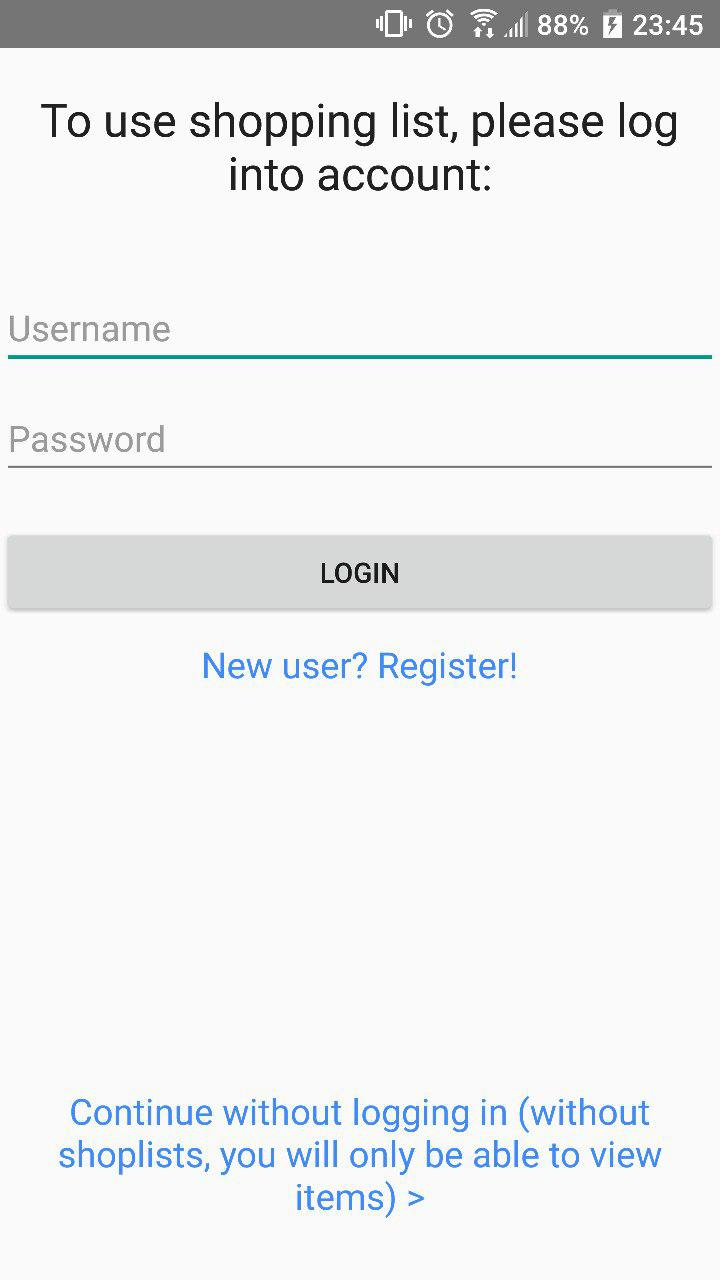
\includegraphics[height=0.42\textheight]{./screenshots/3/login.jpg}
            \caption{\small{Активность для входа в аккаунт пользователя}}
            \label{login_activity}
            \endminipage\hfill
            \minipage{0.45\textwidth}
            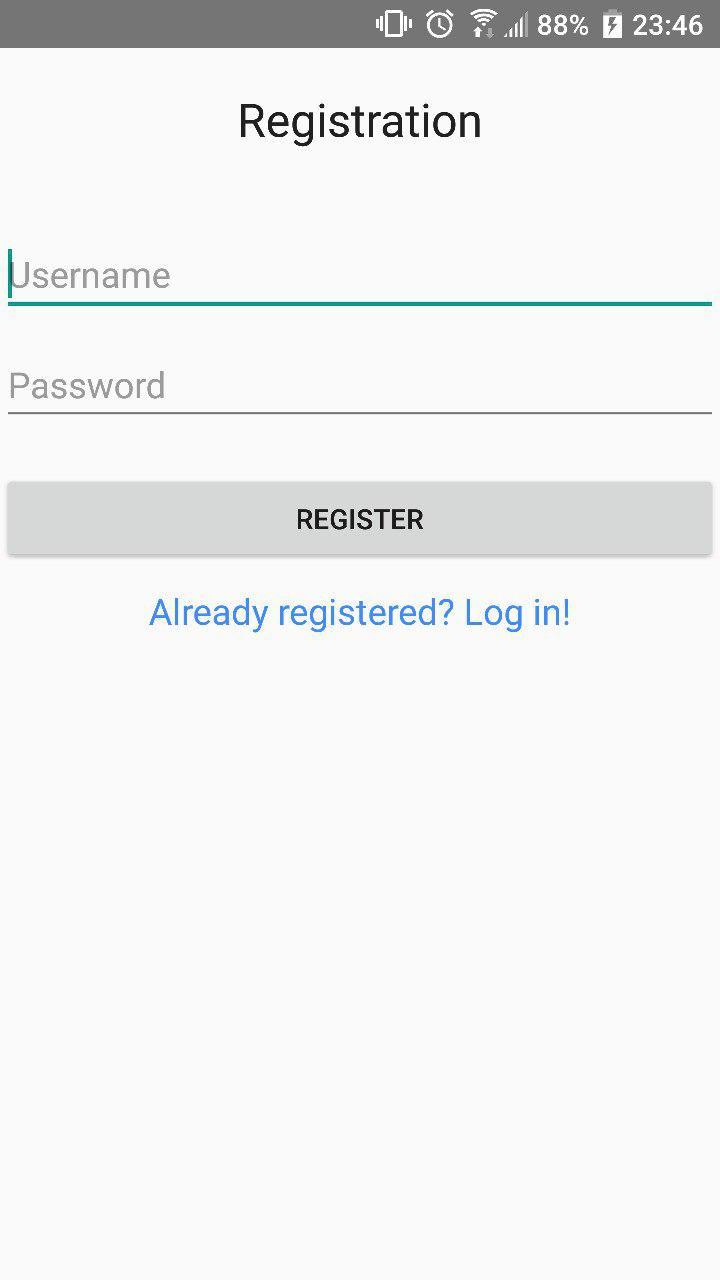
\includegraphics[height=0.42\textheight]{./screenshots/3/register.jpg}
            \caption{\small{Активность для регистрации аккаунта пользователя}}
            \label{register_activity}
            \endminipage
        \end{figure}
    \item \textbf{MainActivity} Главная активность, содержащая 2 дочерних
        фрагмента, toolbar и BottomNavigationView (см. терминологию).\\
        Фрагменты:
        \begin{my_enumerate}
            \item \textbf{HomeFragment} Рис \ref{home_fragment}. Фрагмент, содержащий список всех
                товаров. Список может быть отфильтрован по магазинам и по
                категориям. Содержит toolbar, в котором есть выпадающий список
                для выбора магазина, кнопка для выхода/входа из/в аккаунт(а), и
                меню опций;
            \item \textbf{ShopListsPreviewFragment} Рис \ref{shoplist_fragment}. Фрагмент, содержащий список
                всех списков покупок. Списки покупок упорядочены в виде
                карточек с предпросмотром в них добавленных товаров магазина и
                пользовательских товаров. Нажатие по одному из них открывает
                активность ShopListActivity, содержащюю подробную информацию об
                элементах списка покупок. Долгое нажатие по одному из списков
                вызовет диалоговое окно, в котором спросится подтверждение
                намерения удалить данный список покупок. В элементе toolbar в
                этом фрагменте есть кнопка для входа/выхода в/из аккаунт(а), и
                кнопка для добавления нового списка покупок. Использование
                фрагмента не доступно неавторизованным пользователям;
        \end{my_enumerate}
        \begin{figure}[h!]
            \centering
            \minipage{0.45\textwidth}
            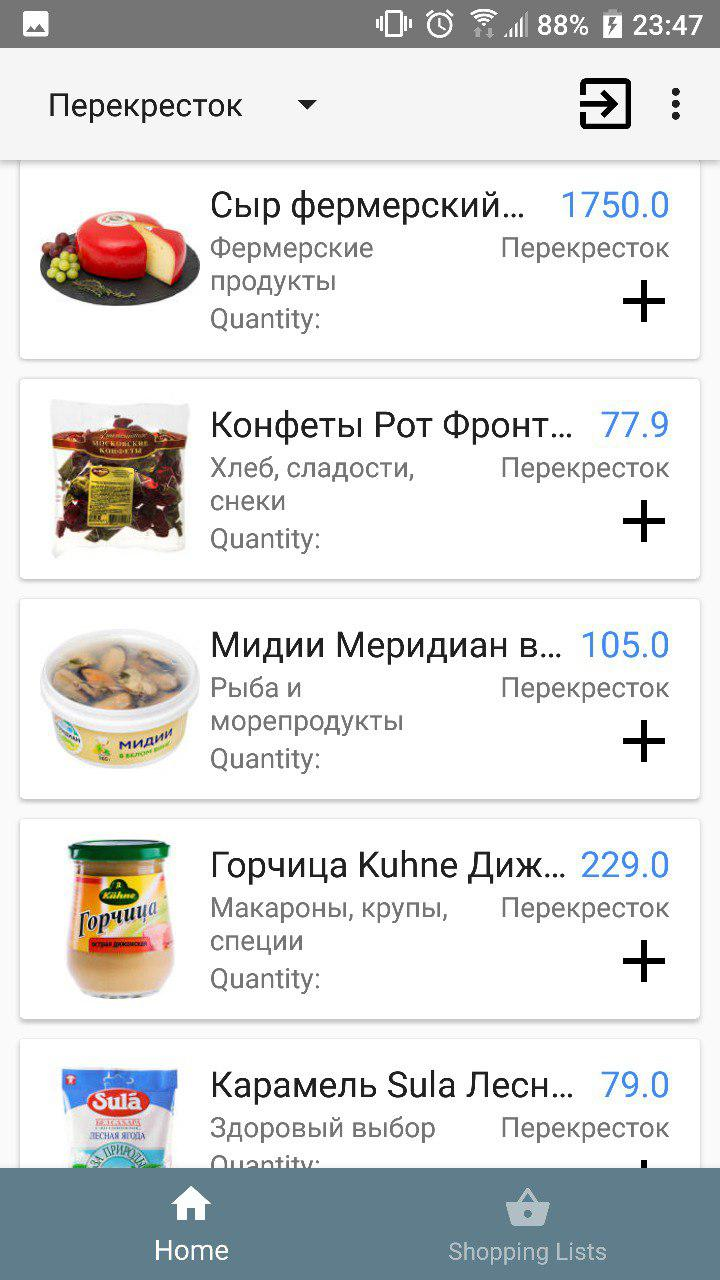
\includegraphics[height=0.42\textheight]{./screenshots/3/home.jpg}
            \caption{\small{MainActivity. Фрагмент со списком товаров магазинов}}
            \label{home_fragment}
            \endminipage\hfill
            \minipage{0.45\textwidth}
            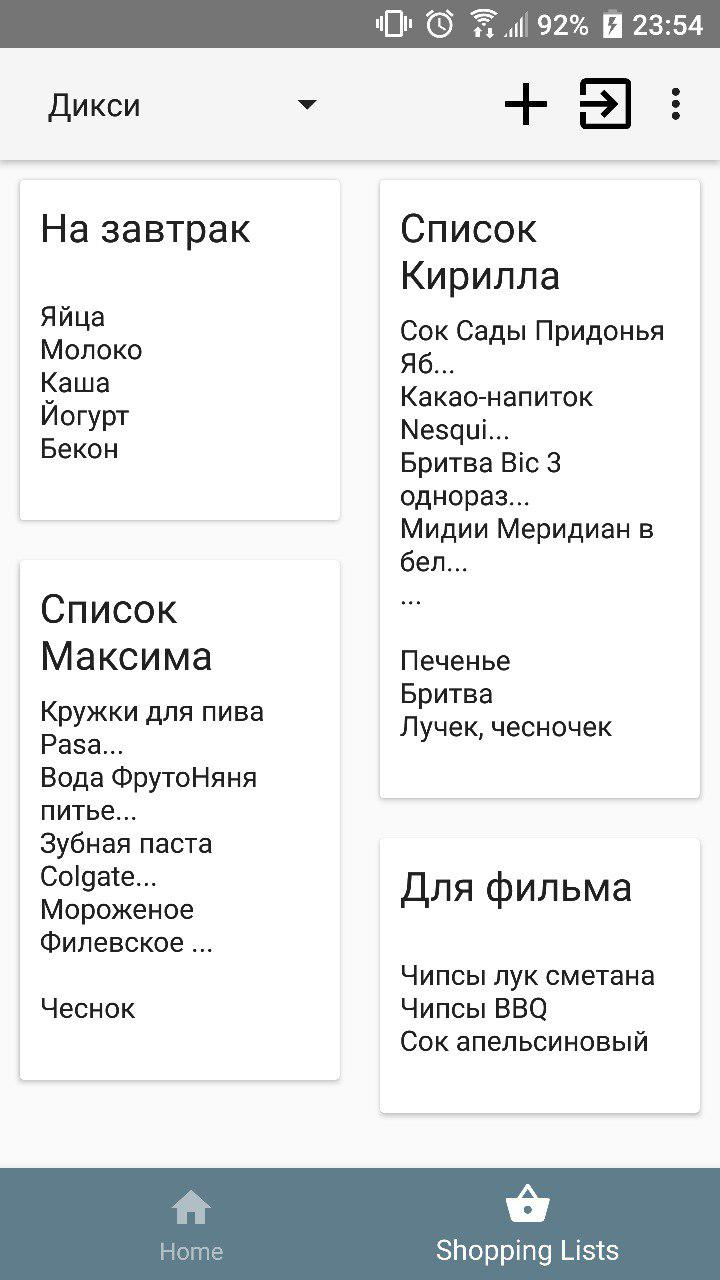
\includegraphics[height=0.42\textheight]{./screenshots/3/all_shoplists.jpg}
            \caption{\small{MainActivity. Фрагмент со всеми списками покупок}}
            \label{shoplist_fragment}
            \endminipage
        \end{figure}
    \item \textbf{ShopListActivity} Рис \ref{shoplist1}, рис \ref{shoplist2}. Активность, содержащая подробную информацию
        о конкретном списке покупок. В элементе toolbar отображается кнопка
        ``назад'', название списка покупок, и итоговая сумма по всем товарам, в
        стандартной для товаров валюте. В центре активности расположен список
        товаров магазина, а под ним - список пользовательских товаров. В свою
        очередь, каждый пользовательский товар содержит список подобранных
        товаров под данный из магазинов. Использование активности не доступно
        неавторизованным пользователям
\begin{figure}[h!]
    \centering
    \minipage{0.45\textwidth}
    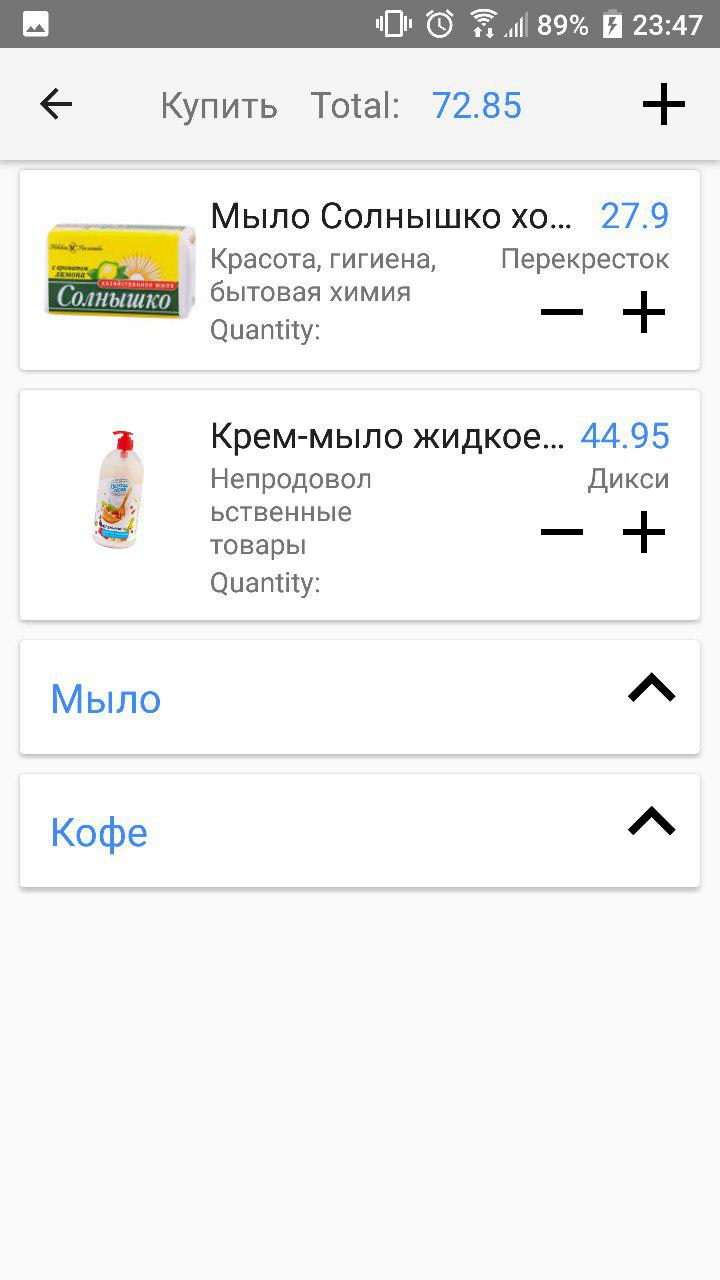
\includegraphics[height=0.42\textheight]{./screenshots/3/shoplist.jpg}
    \caption{\small{ShopListActivity}}
    \label{shoplist1}
    \endminipage\hfill
    \minipage{0.45\textwidth}
    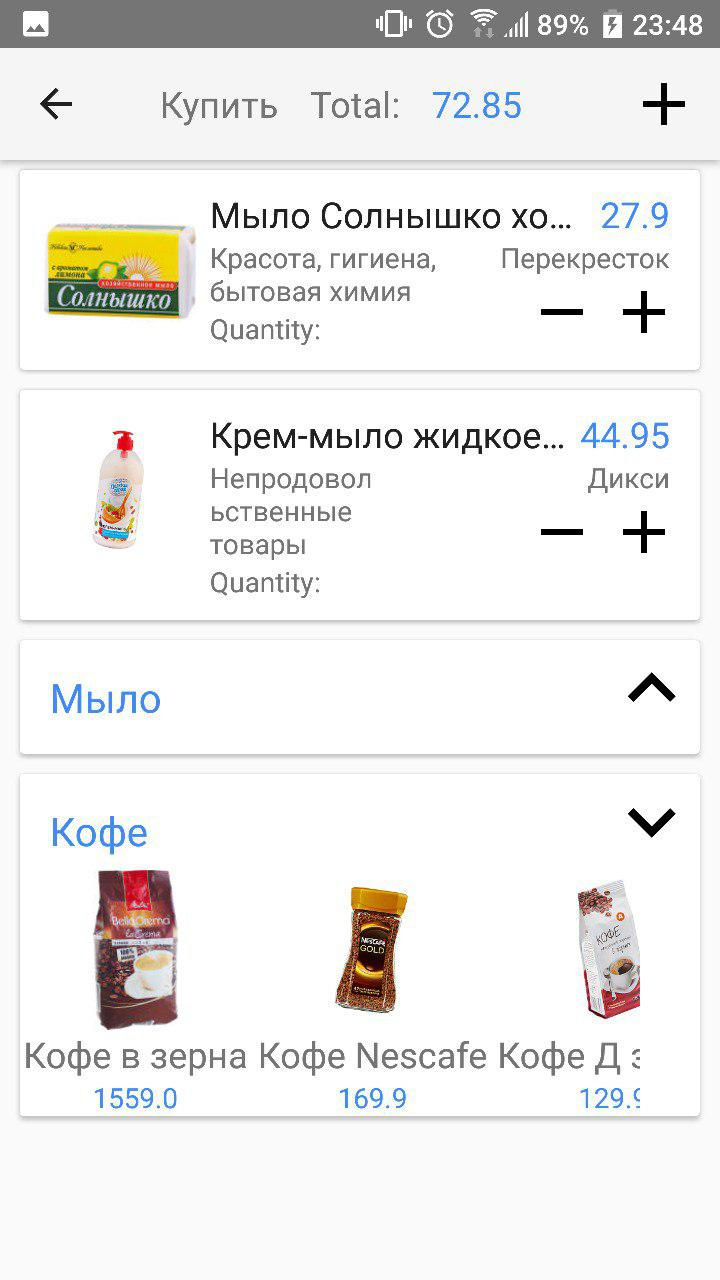
\includegraphics[height=0.42\textheight]{./screenshots/3/shoplist_custom_fold.jpg}
    \caption{\small{ShopListActivity. Показаны соотретствующие пользовательскому товару товары их магазинов}}
    \label{shoplist2}
    \endminipage
\end{figure}
\end{my_enumerate}

\subsubsection{Описание построения crawler'a}

В crawler'e веб-страниц магазинов предусмотрены следующие модули:
spiders/dixy\_spider, spiders/perekrestok\_spider, text\_processor,
dixy\_selectors, perekrestok\_selectors, settings, config, notify и pipelines.\\
\begin{my_enumerate}
    \item \textbf{dixy\_spider} описывает класс DixySpider, унаследованный от
        Scrapy.Spider. Отвечает за получение исходного кода страницы магазина
        ``Дикси'', его парсинга при помощи ``модульных'' xpath селекторов (см.
        терминологию), перехода по страницам на сайте. Формирует объекты классы
        DixyItem и передаёт далее модулю pipelines на обработку;
    \item \textbf{perekrestok\_spider} описывает класс PerekrestokSpider,
        функционал идентичен DixySpider, но действует на сайте магазина
        ``Перекресток'';
    \item \textbf{text\_processor} содержит функции обработки текста при помощи
        регулярных выражений и базовых операций со строками;
    \item \textbf{dixy/perekrestok selectors} содержат соответствующие xpath
        селекторы для веб-страниц магазинов. Выделение этой логики в отдельный
        модуль - корневая причина модульности приложения. В случае изменения
        дизайна сайта, кроулинг которого происходит, админимтратору придётся
        изменить лишь одну строчку для одного элемента на странице;
    \item \textbf{settings, config} содержат настройки и конфигурацию кроулера;
    \item \textbf{pipelines} содержит методы для обработки объектов DixyItem и
        PerekrestokItem. Модуль так же совершает POST запрос на сервер
        приложения для добавления товара в базу данных, и сохраняет все объекты
        в JSON файл
\end{my_enumerate}

\subsection{Ежедневное обновление акций}
Процесс ежедневного обновления акций необходимо проводить, чтобы акции в приложении всегда были актуальными.

На сервере запущена cron job (см. терминологию), котрая каждый день в 2:00 ночи в 6:00 утра запускает процесс кроулинга акций во всех магазинах:

\begin{small}
    \begin{verbatim}
         00 2,6 * * * cd /home/hes/Projects/crawler/easysales && ./crawl_all.sh > /home/hes/crawler.log 2>&1
    \end{verbatim}
\end{small}

Скрипт crawl\_all.sh отвечает за поочередный запуск всех spider'ов. Далее, по
цепочке, спайдеры собирают данные с сайтов при помощи xpath селекторов,
используют модуль text\_processor для очистки собранных данных от non-breaking
space символов, длинных пробелов и других символов. Формируются <Shop>Items,
которые затем отправляются в модуль pipelines. Классы <Shop>Items, процесс
добавления Item'a в базу и модель с селекторами для магазина ``Перекресток''
описаны ниже.

Классы DixyItem и PerekrestokItem унаследованы от EasySalesItem, базового
товара приложения. Его поля всегда заполнены, то есть не могут иметь значения
null.

\begin{small}
    \begin{verbatim}
class EasySalesItem(scrapy.Item):
    name = scrapy.Field()
    newPrice = scrapy.Field()
    imageUrl = scrapy.Field()
    shopId = scrapy.Field()
    crawlDate = scrapy.Field()


class DixyItem(EasySalesItem):
    category = scrapy.Field()
    oldPrice = scrapy.Field()
    discount = scrapy.Field()
    dateIn = scrapy.Field()
    dateOut = scrapy.Field()
    condition = scrapy.Field()


class PerekrestokItem(EasySalesItem):
    category = scrapy.Field()
    oldPrice = scrapy.Field()
    \end{verbatim}
\end{small}

Отправка объекта класса Item в базу данных происходит при помощи API запроса на
сервер:


\begin{small}
    \begin{verbatim}
class DataBaseWriterPipeLine(object):

    def process_item(self, item, spider):
        requests.post(const['ADD_ITEM_API'],
                      data=json.dumps(dict(item)),
                      headers=const['REQUEST_HEADERS'])
        return item
    \end{verbatim}
\end{small}

Xpath селекторы для магазина ``Перекресток''. Модульность и простота использования написанного фрагмента кода достигается тем, что при изменении дизайна сайта магазина, возникает необходимость исправить всего несколько строчек в приведённом фрагменте. Таким образом, частично решается проблема всех кроулеров - поломка, в случае изменения дизайна сайта. А поскольку большинство кроулеров не используют такой модульный подход, времени и сил на починку уходит гораздо больше, так как приходится править множество файлов во многих местах.

\begin{small}
    \begin{verbatim}
# Start urls.
#
URLS = ['https://www.perekrestok.ru/catalog']
URL_CORE = 'https://perekrestok.ru'

# Categiries.
#
CATEGORIES = '//a[@class="xf-catalog-categories__link"]/@href'
CATEGORIES_TEXT = '//span[@class="xf-catalog-categories__text"]/text()'
POST_CATEGORY = '//span[@class="xf-breadcrumbs__current"]/text()'
CURRENT_CATEGORY = '//h1[@class="xf-caption__title"]/text()'

ROOT_NODE = '//ul[@id="catalogItems"]'
ITEM = 'li/div[contains(@class, "xf-product")]'

# Item attributes.
#
NAME = 'div[@class="xf-product__title xf-product-title"]/a[@class="xf-product-\
title__link js-product__title"]/text()'
IMG = 'figure/a/img/@data-src'
NEW_PRICE = 'div/div[contains(@class, "xf-product-cost__current")]/@data-cost'
OLD_PRICE = 'div/div[contains(@class, "xf-price xf-product-cost__prev")]/@data-cost'

# Pagination selector.
#
# next_page = '//li[@class="next"]/a/@href'
NEXT_PAGE = '//a[contains(@class, "xf-paginator__item js-paginator__next")]/@href'
    \end{verbatim}
\end{small}


\newpage
\section{Технико-экономические показатели}
\subsection{Предполагаемая потребность}
«Игра — Эскейп Квест с Использованием Очков Виртуальной Реальности» может быть использована в игровой сфере. Программу могут использовать люди, нуждающиеся как в отдыхе в мире виртуальной реальности, так и желающие интеллектуально развиться в игровой форме.
\subsection{Экономические преимущества разработки}
На момент принятия решения о написании данного продукта во Всемирной сети Интерент был лишь 1 аналог: игра "Lost in the Kismet".
Преимущества данной разработки перед конкурентом:
\begin{my_enumerate}
\item Совместимость со всеми девайсами Cardboard
\item VR Mode и Normal Mode
\item Оригинальный сюжет
\end{my_enumerate}

\newpage
\section{Источники, используемые при разработке}
\subsection{Список используемой литературы}
\begin{my_enumerate}
    \item
    ГОСТ 19.102-77 Стадии разработки. //Единая система программной документации. -М.: ИПК Издательство стандартов, 2001.
    
    \item
    ГОСТ 19.201-78 Техническое задание. Требования к содержанию и оформлению // Единая система программной документации. -М.:ИПК Издательство стандартов, 2001.
    
    \item  ГОСТ 19.404-79 Пояснительная записка. Требования к содержанию и оформлению. //Единая система программной документации. – М.: ИПК Издательство стандартов, 2001
    
    \item
    ГОСТ 19.101-77 Виды программ и программных документов
    //Единая система программной документации. -М.: ИПК Издательство стандартов, 2.: 001.
    
    \item
    ГОСТ 19.103-77 Обозначения программ и программных документов. //Единая система программной документации. -М.: ИПК Издательство стандартов, 2001.
    
    \item
    ГОСТ 19.104-78 Основные надписи //Единая система программной документации. -М.: ИПК Издательство стандартов, 2001.
    
    \item 
    ГОСТ 19.106-78 Требования к программным документам, выполненным печатным способом. //Единая
    система программной документации. – М.: ИПК Издательство стандартов, 2001
    
    \item 
    ГОСТ 19.603-78 Общие правила внесения изменений. //Единая система программной документации. –
    М.: ИПК Издательство стандартов, 2001
    
    \item
    Oculus Documentation [Электронный ресурс]: Режим доступа: https:// developer3.oculus. com/documentation/
    
    \item
    Oculus Developers Blog [Электронный ресурс]: chrispruett – Squeezing Performance out of your Unity Gear VR Game, 2015 - Режим доступа: https://developer3.oculus.com/blog /squeezing-performance-out-of-your-unity-gear-vr-game/
    
    \item 
    Uninty Scripting Reference [Электронный ресурс]: Режим доступа: https: //docs.unity3d. com/ScriptReference/
    
\end{my_enumerate}



\newpage
\section{Приложение 1. Терминология}
\subsection{Терминология}
\begin{description}
  \item[REST (от англ. Representational State Transfer)] -- способ сетевого
    взаимодействия.  REST API определяет набор функций, к которым разработчики
    могут совершать запросы и получать ответы. Взаимодействие происходит по
    протоколу HTTP.  Преимуществом такого подхода является широкое
    распространение протокола HTTP, поэтому REST API можно использовать
    практически из любого языка программирования.
\end{description}



\newpage
\section{Приложение 2. Описание классов}
% При программировании на VueJS, каждый модуль (компонента) предсавляет собой
% отдельный файл, в котором инкапсулированы 

Веб-приложение
\subsection{Discounts.vue}
Поля:\\
\begin{minted}{javascript}
  data: function() {
    return {
      categories: [],
      items: [],
      shoplists: [],
      numPages: 0,
      user: auth.user
    }
  }
\end{minted}
Компонента для отображения списка текущих акций для разных магазинов.

\subsection{Header.vue}
Поля:\\
\begin{minted}{javascript}
  data: function() {
    return {
      shops: [],
      user: auth.user
    }
  }
\end{minted}
Компонента для отображения меню навигации вверху страницы.

\subsection{Item.vue}
Поля:\\
\begin{minted}{javascript}
  data: function() {
    return {
      maxNameLength: 80,
      showImage: true,
      user: auth.user
    };
  },
\end{minted}
Компонента для отображения акционного товара.

%% TODO

\subsection{BellPuzzleLauncher}
Поля:\\
\begin{small}
    \begin{verbatim}
public Transform handMountingPosition;
private bool hasBell = false;
private float angle;
public Transform vrCam;
public GameObject bellPuzzle;
public Transform firstToComplete, secondToComplete;
private bool firstPut = false, secondPut = false;
    \end{verbatim}
\end{small}
Прикрепляется к невидимому кубу с коллайдером, который при столкновении с персонажем и наведении им указателя на место головоломки вешает колокольчик из руки, и, если все 5 на месте, запускает головоломку. 

\subsection{KeyDoorOpener}
Поля:\\
\begin{small}
    \begin{verbatim}
public GameObject door, final;
private static bool opened = false;
private float timeToOpen = 1F;
public Transform handMountingPosition;
    \end{verbatim}
\end{small}

Класс, отвечающий за открытие двери когда в руке у игрока находится ключ.

\subsection{LastPuzzleLogic}
Поля:\\
\begin{small}
    \begin{verbatim}
    char[] numbers;
    bool solved;
    float step;
    string key = "4118956";
    public GameObject Key;
        \end{verbatim}
\end{small}

Класс, отвечающий за поведение последней головоломки с ключем на книжном шкафу.

\subsection{MainMenu}
 Поля:\\
\begin{small}
    \begin{verbatim}
        public GameObject character, story;
   
    \end{verbatim}
\end{small}

Класс главного меню, прикрепляется к двум лэйблам <<PLAY>> и <<EXIT>>.

\subsection{ModChanger}
Поля:\\
\begin{small}
    \begin{verbatim}
    public GameObject modeChooser;
    public static bool vrModeEnabled = false;
    private bool checked_ = false;ы
    \end{verbatim}
\end{small}
Класс, отвечающий за выбор режима (VR Mode или Normal Mode)


\subsection{NumberChanger}
Поля:\\
\begin{small}
    \begin{verbatim}
    int n;
    public float timeDelay = 1F;
    float currentTime = 0F;
    bool gazedAt = false;
    \end{verbatim}
\end{small}
Класс, отвечающий за изменение каждой цифры в последней головоломке.  


\subsection{OpenDoorAndLoadScene}
Поля:\\
\begin{small}
    \begin{verbatim}
    public GameObject door;
    public static bool opened = false;
    public float timeToOpen = 0.6F;
    \end{verbatim}
\end{small}
Класс, отвечающий за открытие двери с TransitScene для входа в дом.

\subsection{PickUpObject}
Поля:\\
\begin{small}
    \begin{verbatim}
    public Vector3 handPosition;
    public Vector3 handRotation;
    Vector3 oldScale;
    public float angle1 = 275F, angle2 = 303F;
    public Transform handMountingPosition;
    public Transform vrCam;
    private bool tilted;
    bool pickedUp = false;
    \end{verbatim}
\end{small}
Класс, отвечающий за перемещение объекта с места, где он лежал, в руку игроку.

\subsection{StoryLogic}
Поля:\\
\begin{small}
    \begin{verbatim}
    public GameObject character, vrCam, guide, tryIt, glhf, stone, constraint;
    private bool freezeMove = true, thrown = false, shown = false;
    \end{verbatim}
\end{small}
Класс, отвечающий за последовательность показа приветственных текстов и обучающего фрагмента вначале.

\subsection{Unscrew}
Поля:\\
\begin{small}
    \begin{verbatim}
    bool unscrewed = false, hasScrewDriver = false;
    public Transform handMountingPosition;
    \end{verbatim}
\end{small}
Класс, отвечающий за откручивание колокольчика со стены при помощи отвертки в руке игрока.

\subsection{VRSlider}
Поля:\\
\begin{small}
    \begin{verbatim}
    public float fillTime = 2f;
    public int Scene = 1;
    private Slider mySlider;
    private float timer;
    private bool gazedAt;
    private Coroutine fillBarRoutine;
    \end{verbatim}
\end{small}
Класс, отвечающий за анимацию слайдера - индикатора внизу экрана.



% Index
\newpage

\eskdListOfChanges

% \phantomsection
% \addcontentsline{toc}{section}{Алфавитный указатель}
% \printindex

\end{document}
